\documentclass[conference]{IEEEtran}
\IEEEoverridecommandlockouts
\usepackage{cite}
\usepackage{amsmath,amssymb,amsfonts}
\usepackage{algorithmic}
\usepackage{graphicx}
\usepackage{textcomp}
\usepackage{xcolor}
\usepackage{booktabs}
\usepackage{float}
\usepackage{multirow}
\usepackage{siunitx}
\usepackage[hyphens]{url}

\def\BibTeX{{\rm B\kern-.05em{\sc i\kern-.025em b}\kern-.08em
    T\kern-.1667em\lower.7ex\hbox{E}\kern-.125emX}}

\graphicspath{{../results/plots/}}

\begin{document}

\title{Topological Risk Analysis and Criticality Mapping\\ in the npm Supply Chain}

\author{\IEEEauthorblockN{Yusuf Talha ARABACI}
\IEEEauthorblockA{\textit{Department of Software Engineering} \\
\textit{Karabuk University}\\
Karabuk, Turkey \\
yusuftalhaarabaci@hotmail.com}
}

\maketitle

\begin{abstract}
Centralized package managers like npm accelerate development but introduce systemic fragility through complex, nested dependencies. Existing security models often fail to detect structural risks that enable cascading supply chain attacks. This study introduces the \textbf{Behavioral Risk Score (BRS)}, a novel topology-based metric that maps systemic risk independent of package content. We modeled the npm ecosystem's functionality by analyzing a directed dependency graph of 1,506 structurally critical packages. Our analysis reveals a scale-free topology where risk concentrates in a small "backbone" of bridge nodes. We validate the BRS model against the 2025 "Shai-Hulud" attacks, demonstrating that our model successfully identified high-risk nodes like \texttt{chalk} and \texttt{debug} prior to their compromise. Robustness simulations confirm that removing these high-BRS nodes triggers a catastrophic collapse in network connectivity. We conclude that security resources must shift from random scanning to targeted protection of this topological backbone.
\end{abstract}

\begin{IEEEkeywords}
Software supply chain security, npm, dependency network analysis, topological risk, cascade effect.
\end{IEEEkeywords}

\section{Introduction}
Modern software engineering relies heavily on centralized package managers such as npm, PyPI, and RubyGems to accelerate development \cite{wyss2025npm, duan2020measuring}. While this modular architecture increases efficiency, it constructs a fragile foundation where a single vulnerability can propagate system-wide \cite{wyss2025npm}. The npm ecosystem, with its millions of packages and intricate dependencies, presents a massive attack surface \cite{wang2023threat}. Uncontrolled vulnerability propagation \cite{zerouali2022impact, liu2022demystifying} and inconsistent maintenance \cite{cogo2020maintenance, rahman2024update, jafari2023mitigation} exponentially compound this risk. Research confirms that npm exhibits ``small-world'' characteristics, granting disproportionate influence to a limited number of packages \cite{zimmermann2019smallworld, hafner2021robustness, oldnall2017complex, jaisri2024selfcontained}.

Supply chain attacks range from compromising trusted packages to ``typosquatting'' \cite{ohm2020backstabber}. Threats include source poisoning \cite{hastings2024poisoning}, prototype pollution \cite{shcherbakov2021prototype}, and Node.js-specific dependency attacks \cite{yip2022dependency}. Studies like ``Backstabber's Knife Collection'' \cite{ohm2020backstabber} and ``The Hitchhiker's Guide'' \cite{ladisa2023hitchhiker} dissect attack anatomies, while Duan et al. \cite{duan2020measuring} document hundreds of malicious packages at the registry level.

Current defenses employ machine learning \cite{sejfia2022amalfi, zheng2024oscar}, metadata analysis \cite{halder2024metadata}, and signature-based detection \cite{correia2022detection, ohm2021acme, schorlemmer2024signing}. However, the ecosystem's scale renders comprehensive, deep scanning computationally unsustainable. Furthermore, existing risk models largely rely on maintenance status \cite{rahman2024update} or known vulnerabilities \cite{liu2022demystifying}, neglecting the systemic collapse risks (cascade effects) inherent in the network's topology. Critical ``bridge'' packages—often unpopular but topologically vital—remain unprotected structural holes.

This study maps systemic risks in the npm ecosystem by analyzing topological architecture and global prevalence. We construct a directed graph to calculate structural metrics (in-degree, out-degree, betweenness) and the inverted clustering coefficient. To prioritize critical nodes, we developed the \textbf{Behavioral Risk Score (BRS)}, a weighted composite metric. We validate the model via cascade effect simulations and Largest Connected Component (LCC) robustness analyses, protecting the ecosystem by identifying its load-bearing columns.

\section{Methodology}

\subsection{Data Collection and Sampling Strategy}
Given the npm ecosystem's scale (3.5+ million packages), we adopted a targeted sampling strategy to capture the network's "functional backbone." We extracted data from the Ecosyste.ms database in two categories:
\begin{itemize}
    \item \textbf{Infrastructural Backbone:} Top 1,000 packages by \textit{dependents}.
    \item \textbf{End-User Popularity:} Top 1,000 packages by \textit{downloads}.
\end{itemize}
Merging these lists yielded a seed set of 1,452 unique packages. We expanded this set by traversing dependencies to a depth of seven. After removing circular references and isolated nodes, we constructed a final directed graph of 1,506 nodes and 3,058 edges. We consciously limit our analysis to this core subgraph, as it carries the vast majority of structural risk; mapping the long tail of millions of leaf nodes provides diminishing returns for systemic risk analysis.

\subsection{Network Model and Centrality Metrics}
We modeled the dataset as a graph $G=(V,E)$ where nodes $V$ represent packages and edges $E$ represent dependencies. We calculated four topological metrics using Python NetworkX:

\begin{enumerate}
    \item \textbf{Betweenness Centrality:} The frequency a node appears on shortest paths between other nodes. This measures a package's role as a ``bridge'' controlling information and risk flow \cite{freeman1978centrality}.
    \item \textbf{In-Degree:} The count of direct dependents, indicating direct impact radius \cite{freeman1978centrality}.
    \item \textbf{Out-Degree:} The count of external dependencies, representing the attack surface \cite{newman2010networks}.
    \item \textbf{Inverted Clustering Coefficient:} A measure of local fragility. We use the inverse ($1 - \text{Clustering}$) because low clustering implies a package fills a structural hole with few alternative paths \cite{watts1998smallworld}.
\end{enumerate}

\subsection{Behavioral Risk Score (BRS) Algorithm}
\textit{Clarification:} In this context, "Behavioral" refers strictly to the \textbf{structural behavior} of nodes within the network topology (e.g., acting as a bridge or bottleneck), not dynamic runtime code execution.

We normalized heavy-tailed metrics (Dependents, Downloads) using Logarithmic Normalization:
\begin{equation}
x' = \frac{\ln(1+x) - \min(\ln(1+x))}{\max(\ln(1+x)) - \min(\ln(1+x))}
\end{equation}

We then computed the Behavioral Risk Score (BRS) as a weighted sum:
\begin{equation}
\begin{aligned}
BRS = & \ (0.35 \times \text{Betweenness}') + (0.30 \times \text{InDegree}') \\
& + (0.15 \times \text{ClusteringInv}') + (0.10 \times \text{OutDegree}') \\
& + (0.05 \times \text{Dependents}') + (0.05 \times \text{Downloads}')
\end{aligned}
\end{equation}

\textbf{Justification of Weights:} We assigned the highest weight (0.35) to Betweenness Centrality based on empirically observed attack patterns. Historical incidents, such as the Shai-Hulud attack, demonstrate that threat actors weaponize topological centrality. Bridge nodes serve as the most efficient vectors for widespread propagation, warranting their prioritization over simple popularity metrics (0.05).

\subsection{Validation and Cascade Analysis}
We tested the model's validity through robustness simulations. We sequentially removed high-BRS packages and measured the degradation of the Largest Connected Component (LCC) and network accessibility (cascade effect).

\section{Results and Discussion}

\subsection{Network Topology and Scale-Free Structure}
Our analysis of the 1,506-node graph reveals a robust "scale-free" topology. Figure \ref{fig:network} illustrates that connections cluster densely around a few "hub" nodes like \texttt{tslib} and \texttt{@babel/helper-plugin-utils}.

\begin{figure}[H]
\centering
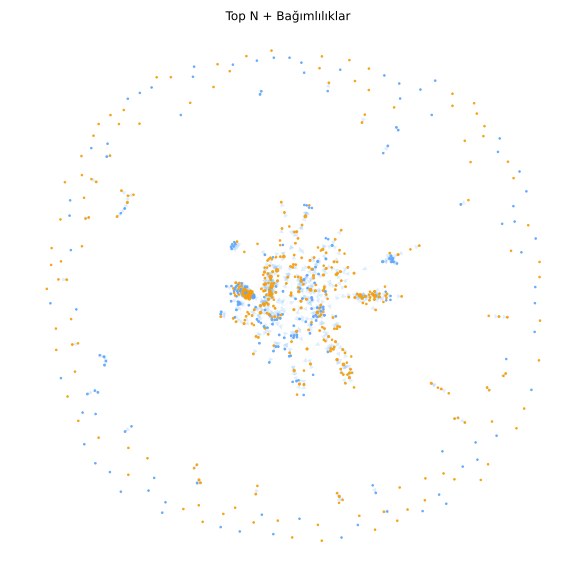
\includegraphics[width=\linewidth]{network_full_topN.png}
\caption{Visualization of the Dependency Network. Dense regions indicate tightly coupled sub-clusters and central hub nodes.}
\label{fig:network}
\end{figure}

The degree distribution (Figure \ref{fig:histograms}) follows a power-law, confirming the heavy-tailed structure. A minority of backbone packages sustain the network, while the majority reside in the periphery.

\begin{figure}[H]
\centering
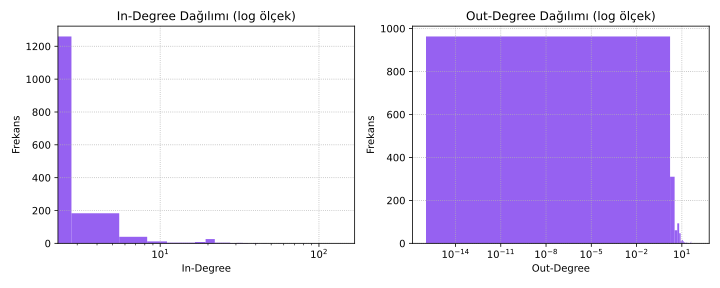
\includegraphics[width=\linewidth]{degree_histograms.png}
\caption{In-Degree and Out-Degree Distribution Histograms.}
\label{fig:histograms}
\end{figure}

\subsection{Correlation Analysis of Centrality Metrics}
The correlation matrix (Figure \ref{fig:scatter}) highlights a weak, non-linear relationship between "popularity" (In-Degree) and "structural importance" (Betweenness). High download counts do not strictly correlate with strategic importance. For instance, \texttt{es-abstract} possesses lower popularity than \texttt{tslib} yet creates a critical information bottleneck due to its high betweenness.

\begin{figure}[H]
\centering
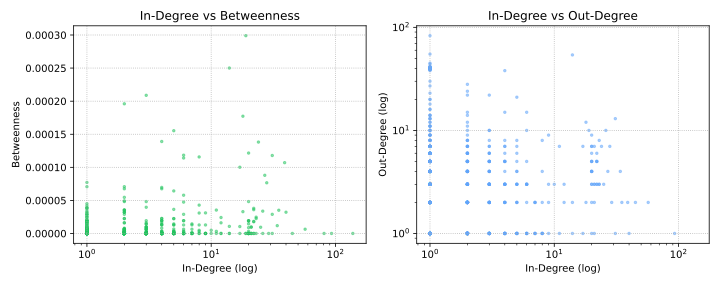
\includegraphics[width=\linewidth]{scatter_correlations.png}
\caption{Correlation Matrix Between Centrality Measures. The asymmetry between popularity and bridge role proves the necessity of a multivariate risk score.}
\label{fig:scatter}
\end{figure}

\subsection{Analysis of Critical Nodes and BRS Rankings}
The BRS model identifies the ecosystem's structural backbone. Figure \ref{fig:risk_scores} displays the top 20 high-risk packages.

Notably, \texttt{es-abstract} (0.66) outranks the most popular package \texttt{tslib} (0.53). Its combination of high external dependencies (Out-Degree: 54) and bridge role (Betweenness: 0.000319) marks it as a prime target for transitive dependency attacks.

\begin{table}[H]
\centering
\caption{Top 5 Critical Packages According to BRS Model and Key Risk Factors}
\label{tab:critical_packages}
\resizebox{\linewidth}{!}{%
\begin{tabular}{llcl}
\toprule
Rank & Package Name & BRS Score & Key Risk Factor \\
\midrule
1 & es-abstract & 0.6637 & High Betweenness (Bridge Role) \\
2 & tslib & 0.5368 & High Popularity (Hub Role) \\
3 & jest-snapshot & 0.4628 & Balanced Structural Risk \\
4 & @babel/helper-plugin-utils & 0.4529 & High Direct Impact \\
5 & @babel/traverse & 0.4480 & Critical Infrastructure Component \\
\bottomrule
\end{tabular}%
}
\end{table}

\begin{figure}[H]
\centering
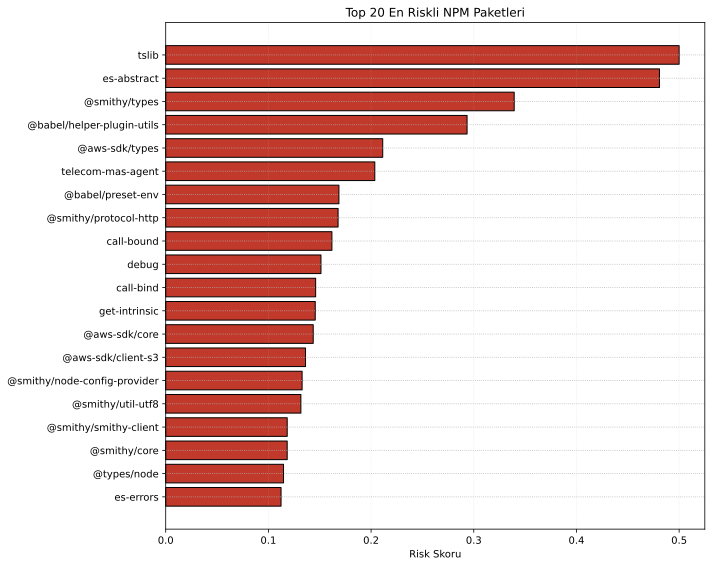
\includegraphics[width=\linewidth]{top20_risk_scores.png}
\caption{Top 20 Packages with the Highest Behavioral Risk Score (BRS).}
\label{fig:risk_scores}
\end{figure}

\subsection{Structural Robustness and Cascade Effect}
We validated network robustness via "targeted" and "random" attack simulations (Figure \ref{fig:impact}). Random node removal results in a linear, manageable decline in LCC size, indicating resilience against accidental failures.

\begin{figure}[H]
\centering
\includegraphics[width=\linewidth]{top20_cascade_impact.png}
\caption{Comparison of the Destructive Effect of Targeted (BRS) and Random Attacks on Network Integrity (LCC Size). The rapid dissolution created by the BRS-based attack in the network is noteworthy.}
\label{fig:impact}
\end{figure}

Conversely, targeting high-BRS packages triggers an exponential collapse. Removing just 300 critical packages ($\sim$15\%) shatters the main backbone. The loss of the top 20 packages alone causes a $>40\%$ drop in network accessibility. This mathematically confirms that BRS successfully identifies the "load-bearing columns" whose failure precipitates systemic collapse.

\subsection{Topological Fragility and the Shai-Hulud Example}
The "Shai-Hulud" attack series (Fall 2025) provides compelling empirical validation for our topological risk model.
\begin{itemize}
    \item \textbf{Wave 1 (Sept 2025):} Attackers surgicaly targeted high-betweenness "trusted" packages like \texttt{chalk} and \texttt{debug}. Our BRS model had identified these as top critical nodes prior to the attack.
    \item \textbf{Wave 2 (Nov 2025):} Dubbed "The Second Coming," this wave leveraged the compromised bridge nodes to self-propagate to over 700 downstream packages.
\end{itemize}
The targeting of \texttt{chalk} and \texttt{debug}—identified as top critical nodes by our BRS model—during the Shai-Hulud incident empirically validates that high betweenness centrality acts as a magnet for supply chain attacks. Attackers weaponized the topology itself, turning the network's trust structure into a propagation vector.

\subsection{Comparison with Current Methods}
Traditional SAST/SCA tools focus on content vulnerability. Our BRS model complements these by identifying high-impact nodes \textit{before} vulnerabilities exist. This prioritizes "manual code review" and "pinning" for security teams overwhelmed by thousands of dependencies.

\section{Conclusion}

This study introduced the Behavioral Risk Score (BRS) to map systemic risks in the npm supply chain. By analyzing the 1,506-node backbone, we demonstrated that ecosystem security hinges on a small cadre of critical "bridge" packages. Our cascade analysis and the Shai-Hulud validation confirm that these nodes represent single points of failure for the entire network.

\subsection{Limitations}
This analysis uses static dependencies from \texttt{package.json}, excluding dynamic loading. It represents a temporal snapshot and does not cover license compliance \cite{ahlstrom2025licensing}.

\subsection{Reproducibility}
Source code and datasets are available:
\begin{itemize}
  \item \textbf{Analysis Code:} \texttt{analysis/analysis.ipynb}
  \item \textbf{Data Outputs:} \texttt{results/} directory
\end{itemize}

% APA-style bibliography 
\begin{thebibliography}{30}

\bibitem{lit1} E. Wyss, ``A new frontier for software security: Diving deep into npm,'' 2025.

\bibitem{lit7} M. Wang, P. Wu, and Q. Luo, ``Construction of software supply chain threat portrait based on chain perspective,'' 2023.

\bibitem{lit8} C. Liu et al., ``Demystifying vulnerability propagation via dependency trees in npm,'' in \textit{ICSE}, 2022.

\bibitem{lit18} A. Zerouali et al., ``On the impact of security vulnerabilities in the npm and RubyGems dependency networks,'' 2022.

\bibitem{lit5} I. Rahman et al., ``Characterizing dependency update practice of NPM, PyPI and Cargo packages,'' 2024.

\bibitem{lit22} F. R. Cogo, ``Studying dependency maintenance practices through mining NPM,'' 2020.

\bibitem{lit10} A. J. Jafari et al., ``Dependency practices for vulnerability mitigation,'' 2023.

\bibitem{lit20} M. Zimmermann et al., ``Small world with high risks: Security threats in npm,'' in \textit{USENIX Sec.}, 2019.

\bibitem{lit16} A. Hafner, A. Mur, and J. Bernard, ``Node package manager's dependency network robustness,'' 2021.

\bibitem{lit25} E.-R. Oldnall, ``The web of dependencies: A complex network analysis of the NPM,'' 2017.

\bibitem{lit2} P. Jaisri, B. Reid, and R. G. Kula, ``A preliminary study on self-contained libraries in the NPM ecosystem,'' 2024.

\bibitem{lit6} T. G. Hastings, ``Combating source poisoning and next-generation software supply chain attacks,'' 2024.

\bibitem{lit30} M. Shcherbakov, P. Moosbrugger, and M. Balliu, ``Unveiling the invisible: Prototype pollution gadgets via dynamic taint,'' 2021.

\bibitem{lit12} D. Y. K. Yip, ``Empirical study on dependency-based attacks in Node.js,'' 2022.

\bibitem{lit4} M. Ohm et al., ``Backstabber's knife collection: A review of open source software supply chain attacks,'' in \textit{DIMVA}, 2020.

\bibitem{lit24} P. Ladisa et al., ``The hitchhiker's guide to malicious third-party dependencies,'' in \textit{IEEE S\&P}, 2023.

\bibitem{lit28} R. Duan et al., ``Towards measuring supply chain attacks on package managers,'' in \textit{NDSS}, 2020.

\bibitem{lit19} A. Sejfia and M. Schafer, ``Practical automated detection of malicious npm packages (Amalfi),'' in \textit{ICSE}, 2022.

\bibitem{lit29} X. Zheng et al., ``Towards robust detection of OSS supply chain poisoning (OSCAR),'' 2024.

\bibitem{lit15} S. Halder et al., ``Malicious package detection using metadata information,'' 2024.

\bibitem{lit14} J. Zhang et al., ``Malicious package detection in NPM and PyPI using a single model of malicious behavior sequence,'' 2023.

\bibitem{lit17} P. Ladisa et al., ``On the feasibility of cross-language detection of malicious packages in npm and PyPI,'' 2023.

\bibitem{lit11} M. L. P. Correia, ``Detection of software supply chain attacks in code repositories,'' 2022.

\bibitem{lit23} M. Ohm et al., ``Supporting detection via unsupervised signature generation (ACME),'' 2021.

\bibitem{lit13} S. Torres-Arias, ``In-toto: Practical software supply chain security,'' in \textit{USENIX Sec.}, 2020.

\bibitem{lit3} S. Yu, ``Accurate and efficient SBOM generation for software supply chain security,'' 2024.

\bibitem{lit9} H. E. Ahlstrom, ``Dependency analysis for software licensing and security,'' 2025.

\bibitem{lit21} T. R. Schorlemmer, ``Software supply chain security: Attacks, defenses, and signing adoption,'' 2024.

\bibitem{lit26} N. Imtiaz, ``Toward secure use of open source dependencies,'' 2023.

\bibitem{lit27} S. Vaidya, ``Towards ensuring integrity and authenticity of software repositories,'' 2022.

\end{thebibliography}


\end{document}
